\documentclass{article}

% External references
\usepackage{pgf}
\usepackage{tikz}
\usepackage{amsmath}
\usepackage{amssymb}
\usepackage{amsthm}
\usepackage{IEEEtrantools}
\usepackage{mathrsfs}

% For the Markov chain diagrams
\usetikzlibrary{arrows,automata}

\title{Resource Allocation Models}
\author{Aaron Geoffrey Sheldon}
\date{\today}
\begin{document}
  \pagenumbering{gobble}
  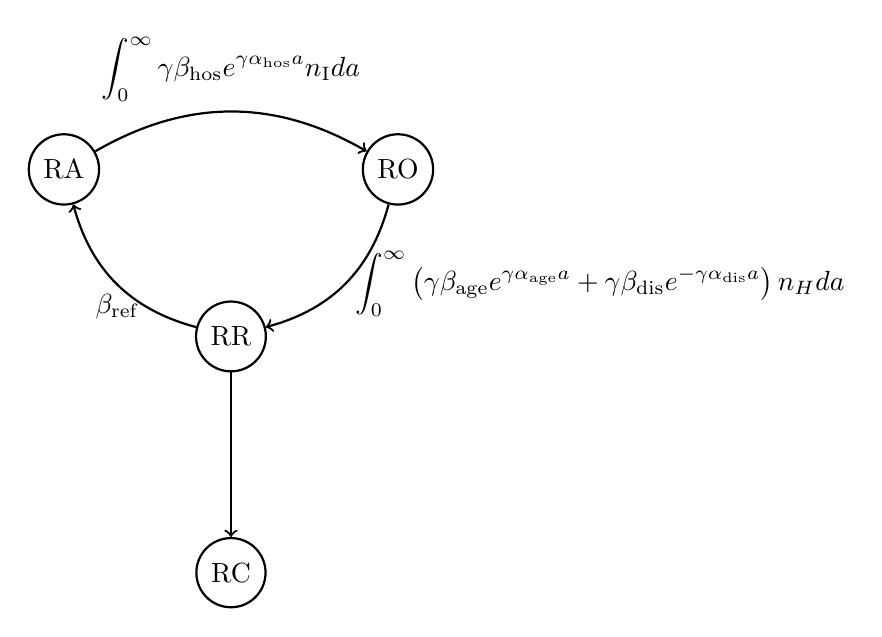
\begin{tikzpicture}[->,thick,node distance=3cm]
    \node[state] (RA)                     {RA};
    \node[state] (RR) [below right of=RA] {RR};
    \node[state] (RO) [above right of=RR] {RO};
    \node[state] (RC) [below of=RR]       {RC};
    \path
      (RA) edge [bend left] node [above] {$\displaystyle\int_0^\infty \gamma\beta_\text{hos} e^{\gamma\alpha_\text{hos} a} n_\text{I} da$} (RO)
      (RR) edge [bend left] node [below] {$\beta_\text{ref}$} (RA)
      (RO) edge [bend left] node [right] {$\displaystyle\int_0^\infty \left(\gamma\beta_\text{age} e^{\gamma\alpha_\text{age} a} + \gamma\beta_\text{dis} e^{-\gamma\alpha_\text{dis} a}\right) n_{H} da$} (RR)
      (RR) edge (RC);
  \end{tikzpicture}
\end{document}